
% SEP 2012 Group 13
% User Manual
%
\documentclass[11pt, a4paper]{report}
\usepackage{graphicx}
\usepackage{fullpage}
\usepackage{url}
\usepackage{xcolor}
\pagestyle{headings}

%%% page parameters
\headsep = 25pt
\usepackage{fancyhdr}
	\pagestyle{fancy}
	\fancyhead{}
	\setlength{\headheight}{15pt}
\fancyhead{\it \small User Manual  \hfill    }

\begin{document}
\oddsidemargin -0.5 cm
\evensidemargin -0.5 cm
\textwidth 15 cm
\topmargin -1.2 cm
\textheight 25 cm
\begin{center}

\includegraphics[scale=1.5]{./UniLogo}\\[1cm]    
\textbf{\Huge \bfseries User Manual}\\[1.5cm]
\textbf{\huge for}\\[0.5cm]


% Title
\textbf{ \huge Archaeology Robot }\\[0.3cm]
\textbf{ \huge Team 13 }\\[2cm]


\begin{tabular}{ |c | p{2cm} |}
	\hline
Yufeng Bai 1600095 & \\[.5cm] \hline
Jun Chen 1206265 & \\[.5cm] \hline
Dawei Geng 1219181 & \\[.5cm] \hline
Yunyao Yao 1203525 & \\[.5cm] \hline
Shikai Li 1214223 & \\[.5cm] \hline
Quang Khoi Nguyen 1187070  & \\[.5cm] \hline
Yatong Zhou 1204471 & \\[.5cm] \hline
\end{tabular}


\vfill

% Bottom of the page
Version 1.0 \\ [0.2cm]
{\large \today}

\end{center}


\tableofcontents



% Version History %

% IMPORTANT %
% Whenever you make a change to this document you MUST put an entry in below
% Must conform to firstName lastName &  date & discription \\ \hline


\clearpage
\section*{Revision History}
\begin{tabular}{| l | l | l | l | }
\hline
Name			& Date			&				&	Version   \\ \hline
Yaoyun Yao		& 7th Oct 2012		&Chapater 1-3, 5-8	&	0.1       \\ \hline
Yatong Zhou	& 17th Oct 2012		&Chapater 4 and error check &	0.1       \\ \hline


\end{tabular}
\clearpage

% Product introduction %

\chapter{Product introduction}
\section{Introduction}
Dear Robot user,\\
Thank you for choosing our product. This user manual is a detailed guide and reference book for the NXT archeology robot of SEP 2012 Group 13. The aim of this user manual is to provide a complete and comprehensive guide to users on the operation of the NXT archeology robot. Please make sure that you read this manual carefully before switching on the robot, it is important to understand the guidelines and instructions before operating the robot.\\
Regards,\\
Yours,\\ 
\flushright SEP 2012 Group 13
\flushleft

\section{Product Summary}
The Lego NXT archeology robot is built and programmed by SEP 2012 Group 13. It was designed to survey an archeology site and to controlled and monitored form a remote Graphical User Interface.  It has the function to survey an archeology site and produce a map which shows the location of any walls above ground, as well as any buried wall and foundations.


\section{Safety Instructions}

\begin{enumerate}
\item Read the user manual carefully before start to operate the robot.

\item The robot was built completely by Lego brick. It is not reinforced in any other way, so be careful while using the robot.

\item To ensure robot works properly, do not try to remove any components. 

\item Do not pull out any cables or change the order of cables.

\item The distance between two wheels are fixed and should not be changed, trying to change the diameter of two wheels will made an effect on movement accuracy.

\end{enumerate}


\pagebreak


% GUI manual %
\chapter{Robot Main Components}

\section{Main Brick}

\begin{center}
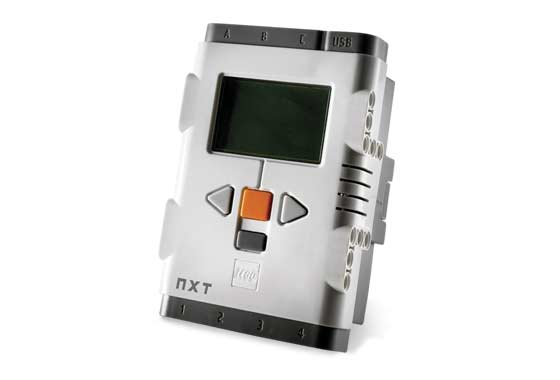
\includegraphics[scale=0.9]{./image/Brick.jpg}\\[0.5cm]
\end{center}
Used to control the motors and to receive signals from sensors. This brick is the brain of the robot. It executes the program in the memory and can send the detected information back to the server side.

\section{Ultrasonic Sensor}

\begin{center}
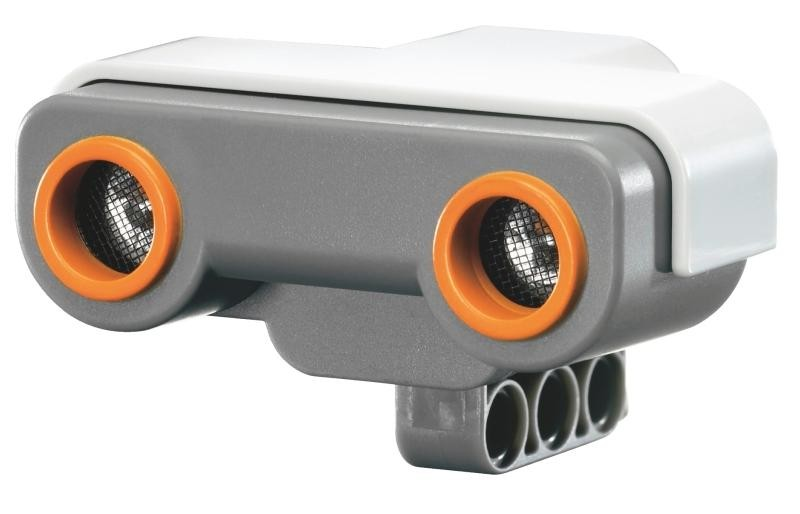
\includegraphics[scale=0.2]{./image/Ultrasonic.jpg}\\[0.5cm]
\end{center}
Used to detect walls and any obstacles. It detects the distance from the obstacle. If ultrasonic sensor find a wall, it will send location information to GUI, and the wall will be displayed on map. 

\section{Light Sensor}

\begin{center}
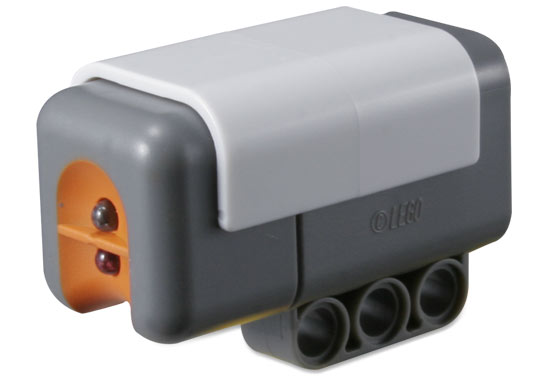
\includegraphics[scale=0.3]{./image/Light.jpg}\\[0.5cm]
\end{center}
Used to scan the map and find hidden walls and no-go zone. It can identify the pixel color on the map by different gray scale.

\section{Motor(3)}
\begin{center}
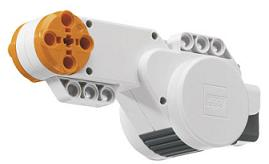
\includegraphics[scale=0.8]{./image/Motor.jpg}\\[0.5cm]
\end{center}
There are totally three motors. Two of them are used to drive the robot wheels, the other one is used to rotate the ultrasonic sensor.






\chapter{Getting Started}

\section{Checklist}

\begin{enumerate}
\item A NXT archeology robot.
\item A USB Cable
\item A USB Bluetooth adapter
\item A Charger
\end{enumerate}


\section{Set The Brick}
To turn the robot on, press the orange button on the brick. Choose "run default" and run, now your robot is ready to receive the command from GUI.


\section{GUI layout}

GUI is consist by several parts:
\begin{center}
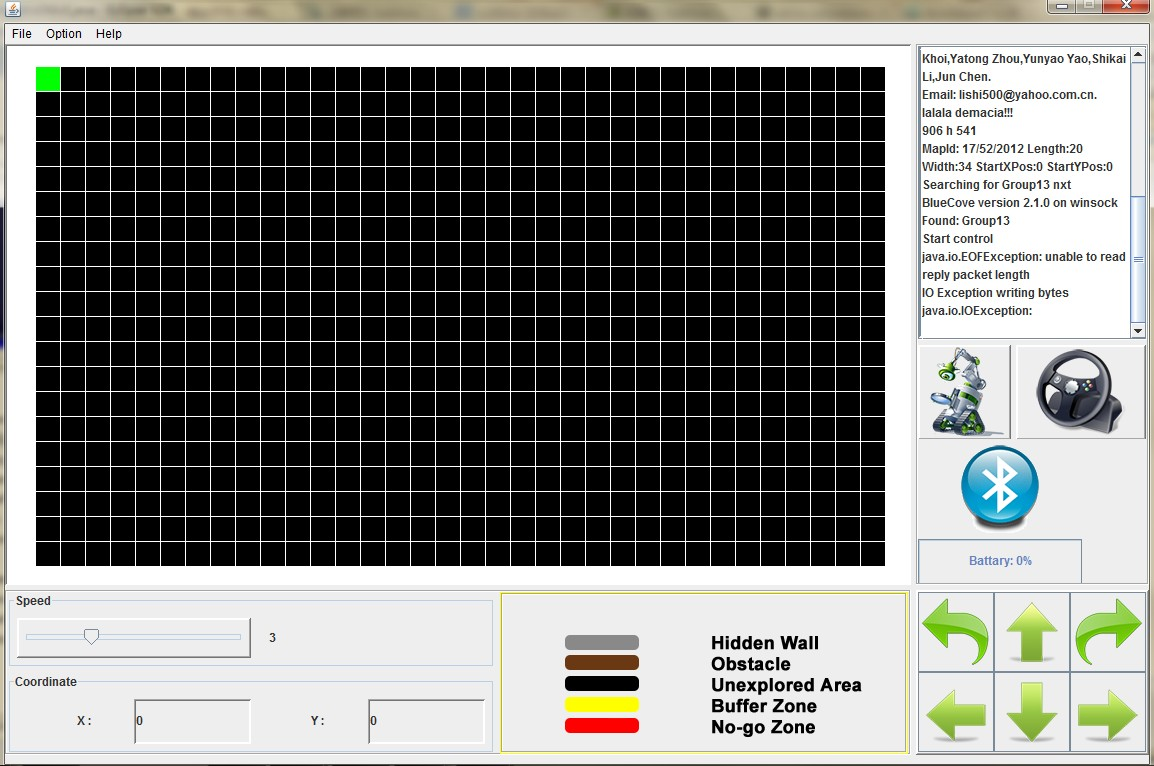
\includegraphics[scale=0.3]{./image/Overview.png}\\[1cm]
\end{center}

\begin{itemize}

	\item Speed control slide bar
	\begin{center}
	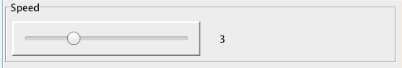
\includegraphics[scale=1]{./image/speed.png}\\[1cm]
	\end{center}
	\item Map display area
	\begin{center}
	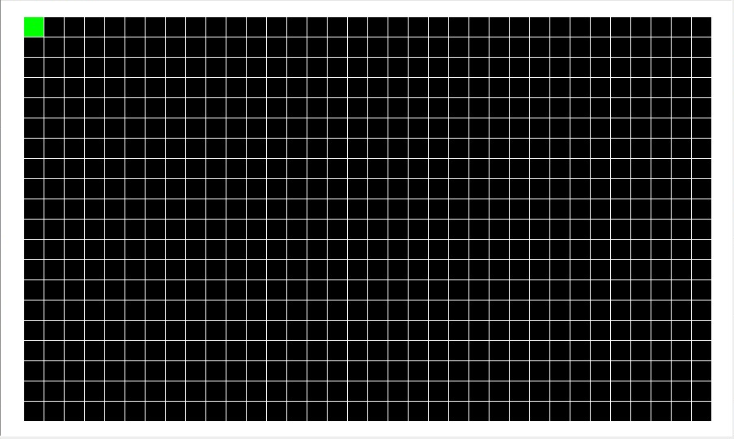
\includegraphics[scale=0.7]{./image/MapArea.png}\\[1cm]
	\end{center}
	\item Bluetooth and battery status
	\begin{center}
	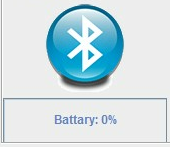
\includegraphics[scale=0.7]{./image/Bluetooth&Battery.png}\\[1cm]
	\end{center}
	\item Control Panel
	\begin{center}
	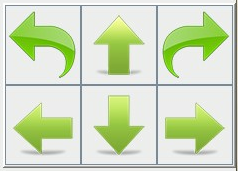
\includegraphics[scale=0.7]{./image/ControlPanel.png}\\[1cm]
	\end{center}
	\item manual mode and automatic mode switch
	\begin{center}
	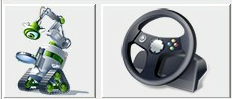
\includegraphics[scale=0.7]{./image/Switch.png}\\[1cm]
	\end{center}
\end{itemize}

\section{Create/Save/Load a Map}


To create a map, user needs to click on "File" from the menu bar and choose "New Map" or press shortcut Ctrl+N, you can also click on the big "Create Map" icon in the map display area. \\
\begin{center}
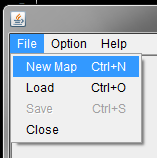
\includegraphics[scale=1]{./image/NewMap.png}\\[0.5cm]
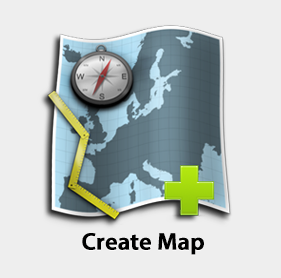
\includegraphics[scale=0.575]{./image/CreateMap.png}\\
\end{center}


Then you will see a pop-up window like this. Enter the Width and Height in Pixel and start point in integer.\\[1cm]
\begin{center}
\includegraphics[scale=1]{./image/MapPanel.png}\\
\end{center}

\noindent\textbf {Note: } As our map consist of 25 x 25 pixels squares, for convenience if you enter a number that is not divide by 25 as Width or Height, it will automatically changed to a largest number that is smaller than your value and divide by 25. For example if you enter 427 as Width, it will create a map with the width 425.\\[1cm]

To save your map as an XML file, select File menu and choose Save or just press Ctrl+S.
\begin{center}
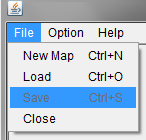
\includegraphics[scale=1]{./image/SaveMap.png}\\[1cm]
\end{center}

To load a map from an XML file, click on "File" and choose "Load"
\begin{center}
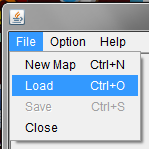
\includegraphics[scale=1]{./image/LoadMap.png}\\[1cm]
\end{center}

\section{Connect GUI to robot}
To connect your robot, click on the Bluetooth icon at right, when the icon is flashing it means it is connecting the robot. When the connection is established the icon will turn blue. It means you can now start to control the robot
\begin{center}

\includegraphics[scale=1]{./image/Bluetooth.png}\\[1cm]
\end{center}
Or you can click on "Option" and choose "Connect the Robot".\\


\noindent\textbf {Note: } Robot must be paired with your computer first. For those computer do not have Bluetooth function, please use the USB Bluetooth adapter we provide which is plug and play.

\section{Mode switch}
There are two control modes to select: manual mode and automatic mode. You can switch between two modes by clicking the mode switch panel. Left is automatic mode, right is manual mode.\\

\paragraph{Manual Mode:}
If manual mode is selected, the robot will not be permitted to move by itself. You can only use GUI control panel to move the robot in this mode. You can switch Automatic Mode by anytime.\\ 

\paragraph{Automatic Mode:}
If automatic mode is selected, the robot will not be permitted to move manually. Robot will automatically travel through the whole map and scan the whole map to GUI. 

\section{Control the robot manually}
There are 6 six kind of movement you can made in manual mode:
\begin{center}
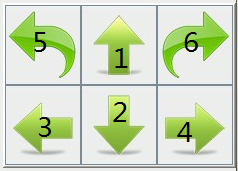
\includegraphics[scale=1]{./image/ControlPanelMark.png}\\[1cm]
\end{center}
\begin{enumerate}

	\item Go forward
	\item Go backward
	\item Turn left
	\item Turn right
	\item Turn left 90 degrees
	\item Turn right 90 degrees
\end{enumerate}
\section{Auto-pilot}
To start auto-pilot, click on automatic mode button. The robot will now start an automatic survey.
\section{Maintainance Mode and User Mode}
By default you are in user mode, to switch to maintainance mode you can click on "Option" and choose "Operation Mode", "Maintainance Mode". In maintainance mode you can set the robot travel speed by yourself.
\begin{center}
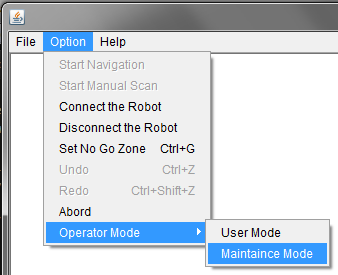
\includegraphics[scale=1]{./image/MainMode.png}\\[1cm]
\end{center}

\section{Speed Control}
By dragging the Speed Control Slider you can control the speed of your robot. You can change speed at both manual mode and automatic mode. 



% Map %
\chapter{Map}

\section{Map introduction}
The map for NXT archeology robot, which is used to represent the archeology site, consists of squares.The width and height of spares are both 25 pixels. Each square with different colors has different meaning which is listed below.
\begin{center}
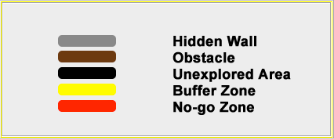
\includegraphics[scale=1]{./image/ColorList.png}\\[1cm]
\end{center}

\section{Zoom in, Zoom out and Drag}
To zoom in and out by scrolling the mouse up and down. To drag the map just click on the map and drag with your mouse.

\noindent\textbf{Note: } The map will only be displayed in the map display area.\\

\section{Mini-Map}
When the map is created or loaded, there is a separate windows on the top-left corner of you screen to display the whole map. This is to give you a overview of the map.


\section{Set No-go Zone}
The map panel on the GUI, which is used to display the discovering map of the archeology site, can be set no go zone by the robot user, this can be activated by click  ``OPTION - SET NO GO ZONE'' or by shortcut Ctrl + G. 

\begin{center}
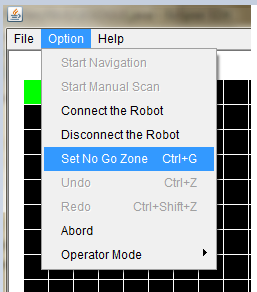
\includegraphics[scale=1]{./image/NoGoZone.png}\\[1cm]
\end{center}

An no-go-zone setting hint comes out and give the user hint about how to set no-go-zone on the map.

\begin{center}
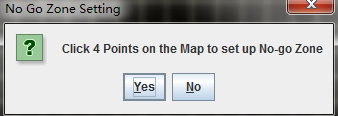
\includegraphics[scale=1]{./image/NoGoZonePop.png}\\[1cm]
\end{center}

Click ``Yes'' if you want to set a no-go-zone. Otherwise, click ``No'' to cancel this operation.
The user should then click four points on the map to make an arbitrary quadrangle. (either convex or concave polygon is acceptable) Before the four positions are chosen, the clicked point will display a light blue point like the following example.

\begin{center}
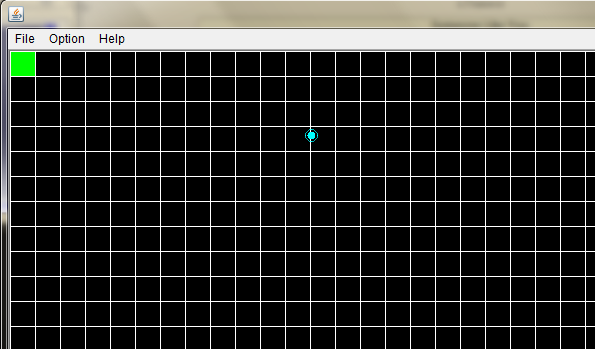
\includegraphics[scale=0.5]{./image/NoGoZoneClick1.png}\\[1cm]
\end{center}



Once the all of the four points are clicked, a quadrangle which is made by the four points will be displayed on the main map panel. The no-go-zone is the area which are drawn as red, and the surrounding yellow colored squares stand for the buffered zone. 

\begin{center}
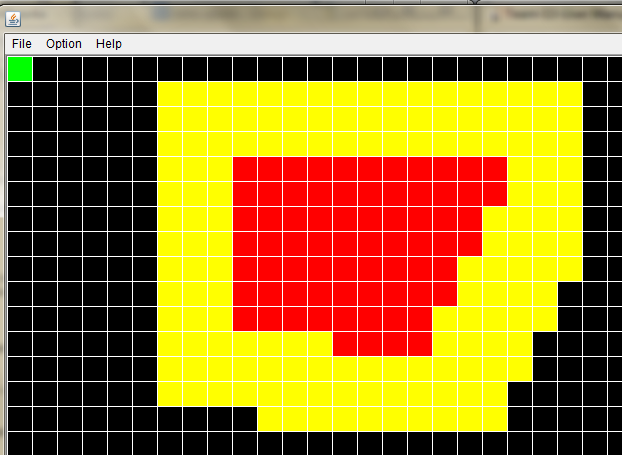
\includegraphics[scale=0.7]{./image/NoGoZoneClick4.png}\\[1cm]
\end{center}

The no-go-zone will be displayed on the mini-map as well. 

\begin{center}
\includegraphics[scale=1]{./image/NoGoZoneMiniClick4.png}\\[1cm]
\end{center}

User can undo the set no-go-zone operation by clicking ``Option-Undo'' or pressing the shortcut ``Ctrl + Z''. More no-go-zone can be added like this way. 


\chapter {Operation Modes}

\section{Manual Control Mode}
When the robot is connected, and user press the Manual Control Model button in the GUI, the robot enters the Manual Control. User can move robot manually with pressing the ``Up, Down, Left, Right'' buttons to anywhere on the map. However, the map will not be scanned in this mode, that is, any information on the map will not be transferred and displayed on the GUI.
%%%%%%%%picture

\section{Manual-scan Mode}
User can change the robot to Manual-scan Mode when the robot is connected, in this mode, the robot can scan the map manually after press the Option-Start Manual-scan on the menu bar. In this mode, the robot can be controlled by the user, each movement of the robot will let the robot scan the current pixel information, transfer to the host and display on the map panel of GUI
%%%%%%picture

\section{Auto-scan Mode}
User can change the robot to auto Mode when the robot is connected, in this mode, the robot can scan the map automatically after press the Option-Start Navigation on the menu bar.
%%%%%%%picture









\chapter{Robot Function}


\section{Detect Walls}
Robot is able to detect a wall in manual mode and automatic mode and map the wall on GUI by using the ultrasonic sensor at front. When a wall is detected in manual mode robot will stop moving forward even the user force it to. In automatic mode if a wall is detected the robot will avoid the wall and continuing searching the map.\\


\noindent\textbf{Note: } Robot can only detect a wall that is higher that the ultrasonic sensor.


\section{Indicate No-go zone}
The Robot can find No-go zone by using the light sensor at the front. When robot find a no-go zone it will be displayed on the map, the corresponding node will be marked as red.

\section{Path Finding}
Robot can find a path avoiding all the obstacles and finally travel through all the nodes on the map.

\noindent\textbf{Note: } In some complicated area you can always use manual control to help the robot go through the map faster.



\chapter {System Requirements}

\section {Windows/Linux/Mac OS with 32-bit JRE}
As our program is coded in JAVA, devices used to control the robot must have the capability to run JAVA programs. Also you must install Lejos.\\

\noindent\textbf {To download the latest version of JRE click here:}\\

\noindent{\color{blue} http://www.oracle.com/technetwork/java/javase/downloads/index.html}\\

\noindent\textbf{Note: } We strongly suggest you to download the 32-bits version of the JRE even you are running on a 64-bits machine. As it is more compatible with Lejos.\\[1cm]


\section {Fantom driver for The LEGO Mindstorms}
Fantom is a compulsory driver for installing leJOS NXJ Version 0.9.1 beta.\\
\noindent\textbf {To get the corresponding Fantom driver, please go to:} \\[0.2cm]
{\color{blue} http://mindstorms.lego.com/en-us/support/files/Driver.aspx} \\[0.5cm]
Download and install it.\\[1cm]

\section {leJOS NXJ Version 0.9.1 beta}
LeJOS NXJ is a necessary plug-in for Java Eclipse\\[0.2cm]
\textbf {To get the latest version of Lejos click here:}\\

\noindent{\color{blue} http://lejos.sourceforge.net/rcx-downloads.php}\\[0.5cm]
Download and install it.\\[1cm]

\section {Apache Ant and GNU Make}


\chapter{Getting Started}

\section{How to Install}
Install the program using Apache Ant and GNU Make\\
\section{Start Using}
\begin{enumerate}

	\item Prefaration before operation
	\item Switch on the robot,run Bobot Server.
	\item Open host program (Make sure bluetooth is on)
	\item Create a new map or load an existing map from your computer
	\item Connect the GUI with the robot
	\item Start manual control to get to starting point
	\item Switch to auto-scan or manual-scan
	\item Stop or resume the operation...
	\item Operation Complete
	\item Save the map
\end{enumerate}



\pagebreak
 



\chapter{FAQ}

\section{Why is the robot can not be turned on?}
Ensure the battery is charged, then try to turn on the robot again.

\section{Why is Bluetooth connection can not be made?}
Before trying to connect the robot with GUI make sure the brick has paired with your computer. 4 digit pairing code can be set on the brick which is set to 0000 by default.

\section{How would I know my robot is on?}
If you successfully turn on the robot by pressing the orange button on the brick, you hear a sound. Otherwise you robot maybe run out of battery.


\section{How would I know if the Bluetooth is connected?}
If the Bluetooth icon on GUI is blue rather than gray, Bluetooth connection is established.


\section{Can I use USB to connect robot}
You can NOT connect your robot will USB, GUI only support Bluetooth connnection.

\section{How can I exit the program on robot?}
If you close the GUI window on you computer, the robot will exit and restart.

\section{What should I do if the robot program crashed?}
If your robot has no response to the GUI, the program maybe crashed. You can poll out the battery pack at the back, then put it back, the robot will be restarted.

\chapter{Glossary}


\paragraph{GUI:} Acronym of Graphic User Interface. This is what is used to display map and control panel

\paragraph{Control Panel:} The manual control panel.

\paragraph{No-Go Zone:} A zone which the robot is forbidden to enter.

\paragraph{Pixel:} The smallest addressable element in a display device.

\paragraph{Square:} The smallest addressable element in the map.

\paragraph{Lejos:} A firmware replacement for Lego Mindstorms programmable bricks, which allows Lego Mindstorms robots to be programmed in the Java programming language.


\pagebreak{}






\end{document}

